% TikZ Figure: Shadow IT Decay Function (Psi)
% Standalone LaTeX file for generating PDF figure
\documentclass[tikz,border=5pt]{standalone}
\usepackage{pgfplots}
\pgfplotsset{compat=1.18}
\usepackage{amsmath}

\begin{document}
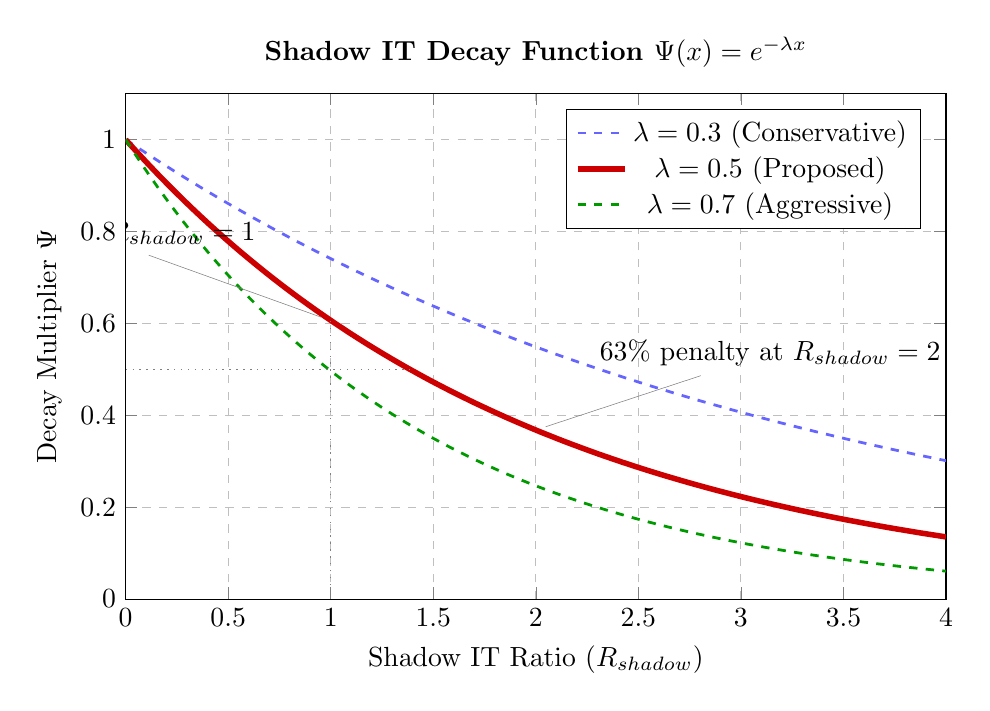
\begin{tikzpicture}
\begin{axis}[
    title={\textbf{Shadow IT Decay Function $\Psi(x) = e^{-\lambda x}$}},
    xlabel={Shadow IT Ratio ($R_{shadow}$)},
    ylabel={Decay Multiplier $\Psi$},
    xmin=0, xmax=4,
    ymin=0, ymax=1.1,
    xtick={0,0.5,1,1.5,2,2.5,3,3.5,4},
    ytick={0,0.2,0.4,0.6,0.8,1.0},
    legend pos=north east,
    ymajorgrids=true,
    xmajorgrids=true,
    grid style=dashed,
    width=12cm,
    height=8cm,
]

% Lambda = 0.3 (Conservative)
\addplot[
    domain=0:4,
    samples=100,
    color=blue!60,
    line width=1pt,
    dashed,
]
{exp(-0.3*x)};
\addlegendentry{$\lambda = 0.3$ (Conservative)}

% Lambda = 0.5 (Default - Proposed)
\addplot[
    domain=0:4,
    samples=100,
    color=red!80!black,
    line width=2pt,
]
{exp(-0.5*x)};
\addlegendentry{$\lambda = 0.5$ (Proposed)}

% Lambda = 0.7 (Aggressive)
\addplot[
    domain=0:4,
    samples=100,
    color=green!60!black,
    line width=1pt,
    dashed,
]
{exp(-0.7*x)};
\addlegendentry{$\lambda = 0.7$ (Aggressive)}

% Key annotation points
\node[pin={[pin distance=1cm]135:{40\% penalty at $R_{shadow}=1$}}] at (axis cs:1,0.606) {};
\node[pin={[pin distance=0.8cm]45:{63\% penalty at $R_{shadow}=2$}}] at (axis cs:2,0.368) {};

% Vertical line at R_shadow = 1
\addplot[
    color=gray,
    line width=0.5pt,
    dotted,
] coordinates {(1,0) (1,0.606)};

% Horizontal line at Psi = 0.5
\addplot[
    color=gray,
    line width=0.5pt,
    dotted,
] coordinates {(0,0.5) (1.386,0.5)};

\end{axis}
\end{tikzpicture}
\end{document}
